\chapter{Collision Data Samples}
\label{chap:data}
\section{Data Periods and Good Run List}
\label{EventSel:GRL}

\indent This analysis uses the LHC proton-proton collision data at a centre-of-mass energy of $\sqrt{s}$=13 TeV that was collected by ATLAS in 2015 and 2016. \\

\indent We select data where all relevant subdetector parts are running without defects and the quality of data is good.  This is done by requiring the data pass a good run list (GRL).  The good run list is compiled from data that pass manual and automated checks on both detector hardware and the kinematics of reconstructed physics objects.  \\

\indent The GRLs used for the 2015 dataset is {\tt \scriptsize data15\_13TeV.periodAllYear\_DetStatus-v79-repro20-02\_DQDefects-00-02-02\_PHYS\_StandardGRL\_All\_Good\_25ns.xml}.  \\
\indent The GRL for the 2016 data is {\tt \scriptsize data16\_13TeV.periodAllYear\_DetStatus-v83-pro20-15\_DQDefects-00-02-04\_PHYS\_StandardGRL\_All\_Good\_25ns.xml}.

\indent The dataset after GRL selection corresponds to a total integrated luminosity of $\intlumi \pm 1.15$ $\ifb$.  The total integrated luminosity as a function of time for 2015 and 2016 before the requirement of an GRL is shown in figure \ref{fig:data2015-2016}.\\

\begin{figure}[htb]
  \begin{center}
    \begin{subfigure}[a]{0.45\textwidth}
        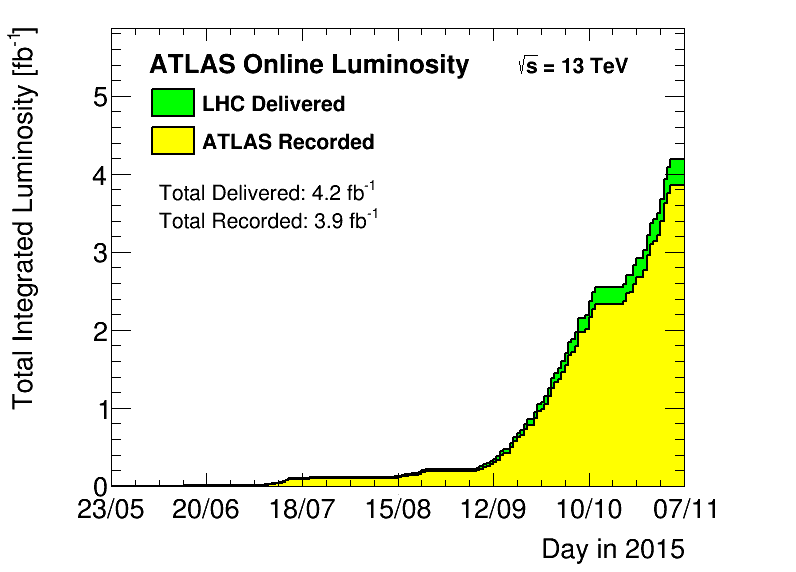
\includegraphics[width=\textwidth]{figures/Data/IntLumi2015.png}\hspace{0.05\textwidth}
                \caption{ }
    \end{subfigure}
    \begin{subfigure}[b]{0.45\textwidth}
        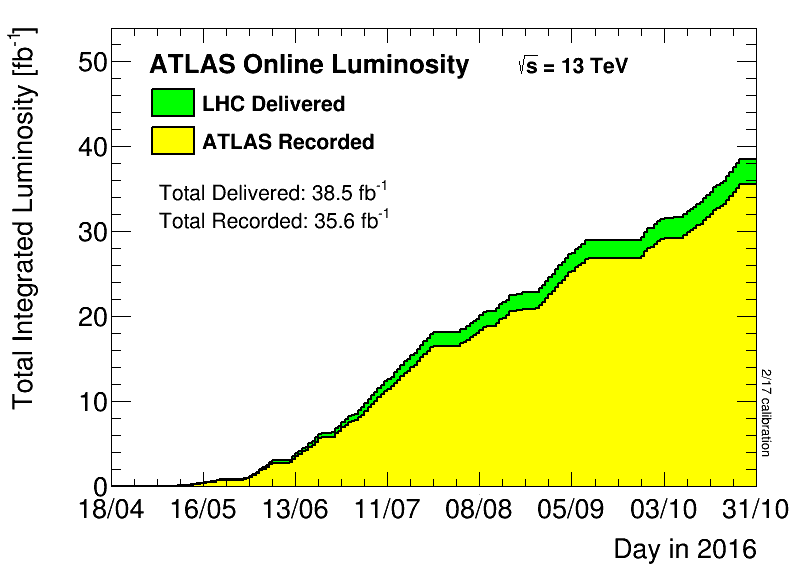
\includegraphics[width=\textwidth]{figures/Data/IntLumi2016.png}\hspace{0.05\textwidth}
                \caption{ }
    \end{subfigure}
\end{center}
\caption{Distribution of the amount of data delivered by the LHC and recorded by ATLAS vs time in 2015 (a) and 2016 (b) }
\label{fig:data2015-2016} 
\end{figure}

\indent Peak luminosity reached $1.38 \times 10^{34}$  cm$^{-2}$ sec$^{-1}$ in 2016.  Taking data at this high rate means we expect multiple p-p interactions in every bunch crossing.  The average number of interactions per bunch crossing, $\braket{\mu}$, is 13.7 in 2015 and 23.2 in 2016.  The distribution of the mean number of interactions per bunch crossing is given in figure \ref{fig:nVtx}.   \\

\begin{figure}[htb]
  \begin{center}
    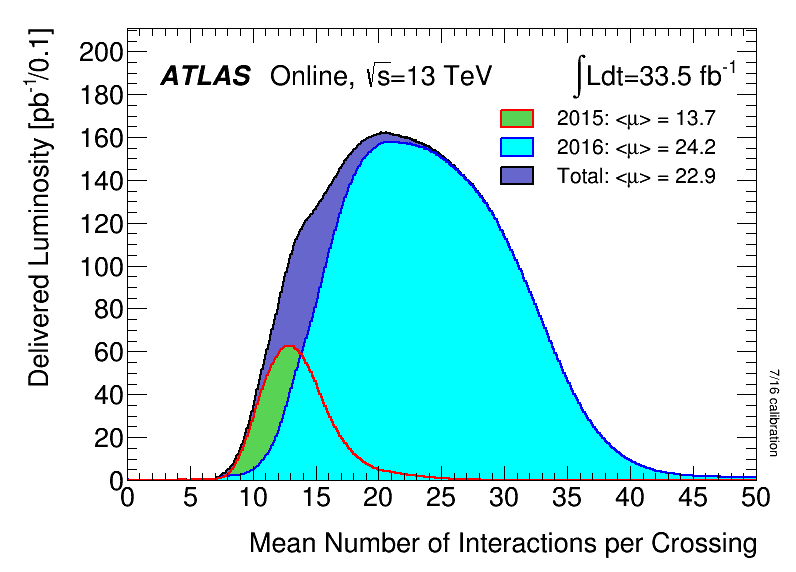
\includegraphics[width=0.75\textwidth]{figures/Data/mu_2015_2016_LHCC.png}\hspace{0.05\textwidth}
\end{center}
\caption{Distribution of the mean number of interactions per bunch crossing weighted by integrated luminosity for 2015 and 2016 ATLAS data taking.    }
\label{fig:nVtx} 
\end{figure}

\indent In order to keep data flow to a manageable size, ATLAS only records events if a trigger is fired.  The ATLAS trigger system is summarized in chapter \ref{chap:trigger}.  This analysis uses the lowest unprescaled $\met$ trigger for each data taking period.  This trigger threshold was set at 70 $\gev$ to 110 $\gev$ depending on the data taking period. The trigger efficiency curve as a function of offline $\met$ for select $\met$ triggers can be seen in figure \ref{fig:trigTurnON}. \\

\chapter{Event Preselection}
\label{chap:Selection_EventPreselection}

\indent After requirements on the Good Run List described in section \ref{EventSel:GRL}.  We require that the event pass a few basic selections to ensure that the events do not have large amounts of calorimeter noise or non-collision backgrounds.  These basic selections are applied to all control regions (CR), validation regions (VR), and signal regions (SR).  Together these basic selections are referred to as event cleaning and jet cleaning.  \\

\indent A brief description of the preselection requirements is given below: Details on all object definitions can be found in chapter \ref{chap:objects}. \\

\begin{description}
\item[Cut 1] Data events must be in accepted according to the Good Runs List (GRL) described in chapter \ref{EventSel:GRL}.  This ensures all relevant subdetector of ATLAS are operating normally during data taking. 
\item[Cut 2] Remove events with noise bursts and possible incomplete events due to the TTC reset procedure from the data. Data events must have no error flags in the calorimeter and ID.  The following error flags must be set to zero: larError $== 0$, tileError $== 0$, SCT error $==0$, and coreFlags $\&0x4000 == 0$.
\item[Cut 4] Require that at least one reconstructed primary vertex must exist.
\item[Cut 5] Events must not contain any {\tt BadLoose} jets with $\pT > 20 \gev$ (at any \eta\ range). Bad quality jets indicate the presence of calorimeter noise or non-collision backgrounds. Both can lead to poor $\met$ reconstruction. Hence, the whole event is rejected.  {\tt BadLoose} jets are defined in jet quality selection in section \ref{sec:jet:quality}.  
\item[Cut 6] The event must not contain any cosmic muons.  Cosmic muons are identified as muons with large impact parameters  ($|z_0| > 1$ mm and $|d_0| > 0.2$ mm).  Only {\tt Baseline} muons after overlap removal are considered in cosmic muon identification.
\item[Cut 7] The event must not contain any muons with $?(q/p)/|(q/p)| > 0.2$.  Muons with large fractional uncertainty often result from kaon decays or poorly reconstructed inner detector tracks that are incorrectly matched to muon spectrometer segments. These muons may result in misreconstructed $\met$ so the whole event is rejected.
\end{description}

\indent On top of these basic requirements, additional preselection requirement are applied to each CR, VR and SR depending on the number of leptons required in the respective region.  \\

\section{Zero Lepton Pre-Selection}

\indent Any zero lepton region requires the selections given in table \ref{tab:0Lcommon}. \\

\begin{table}[htbp]
  \begin{center}
    \begin{tabular}{l|c} \hline\hline
      \multicolumn{2}{c}{GRL, Event Cleaning and Jet Cleaning} \\ \hline
      \multicolumn{2}{c}{$\met$ Trigger}   \\ \hline
      $\met$ & $> 250\GeV$ \\ \hline
      $N_{\rm{{\tt Baseline}~lep}}$ & 0 \\ \hline
      \antikt\ $R=0.4$ {\tt Signal} jets & $\ge 4,~\pt>80,80,40,40 \gev$ \\ \hline
      $b$-tagged {\tt Signal} jets & $\ge1$ \\ \hline
      % $\dphijettwomet$ & $> \pi/5$ \\ 
      $\dphijettwomet$ & $> 0.4$ \\ 
              & \\ [-2.5ex] \hline
      $\mettrk$  & $> 30 \gev$ \\ \hline 
      % & \\ [-2.5ex]
      $\dphimettrk$ & $<\pi/3$ \\ \hline
      % & \\ [-2.5ex] \hline
      % $\tau$ veto & yes \\ \hline
      % $\mtbmetmindphi$ & $> 175 \gev$ \\ \hline \hline
    \end{tabular}
  \caption{ Zero lepton preselection criteria common to all zero lepton signal and validation regions.}
  \end{center}
  \label{tab:0Lcommon}
\end{table}

\indent All zero lepton regions trigger on $\met$ using the lowest unprescaled $\met$ trigger for that data period.  An offline selection of $\met > 250 \gev$ is required to ensure that all accepted events are on the trigger efficiency plateau.  The trigger efficiency curve as a function of offline $\met$ for select $\met$ triggers can be seen in figure \ref{fig:trigTurnON}.  \\

\indent We require that the event contains exactly zero {\tt Baseline} leptons.  We also require at least four {\tt Signal} jets with a minimum $\pt$ of $(80,80,40,40) \gev$ in the event.  At least one {\tt Signal} jet must be b-tagged at the 77 percent working point.  These jet energy and multiplicity requirements are loose and will be superseded by more stringent selections in the SR, VRs and CRs.  \\

\indent For our analysis the primary reason that QCD multijet background is able to pass the SR selections is due to misreconstructed jets.  QCD multijet produces little intrinsic $\met$.  In order to pass the 250 $\gev$ $\met$ requirement, multijet background need additional fake $\met$ from mis-measured jets.  For example, an extremely energetic jet may punch through the calorimeter and be reconstructed with a small $E_T$.  This lost $E_T$ maybe reconstructed as $\met$.  \\

\indent The $\dphijettwomet > 0.4$ requirement ensures that the $\met$ is not collinear with the most energetic jets in the event.  This provides strong rejection against fake $\met$ resulting from a single misreconstructed energetic jet.  Requirements on a loose agreement between $\met$ and $\mettrk$ also discriminate against $\met$ resulting from misreconstructed jets and therefore QCD multijet. \\

\section{One Lepton Pre-Selection}

\indent The one lepton preselection is similar to the zero lepton preselection except for several important requirements.  The one lepton preselection is summarized in table \ref{tab:1Lcommon}. \\

\begin{table}[htbp]
  \begin{center}
    \begin{tabular}{l|c} \hline\hline
      \multicolumn{2}{c}{GRL, Event Cleaning and Jet Cleaning} \\ \hline
      \multicolumn{2}{c}{$\met$ Trigger} \\ \hline
      $\met$ & $> 250\GeV$ \\ \hline
      $N_{\rm{{\tt Signal}~lep}}$ & 1 \\ \hline
    $N_{jets}$ & $\ge 4$ \\ \hline
      $b$-tagged {\tt Signal} jets & $\ge1$ \\ \hline
      $\dphijettwomet$ & $> 0.4$ \\
              & \\ [-2.5ex] \hline
    \end{tabular}
  \caption{ One lepton pre-selection criteria common to all one lepton signal and validation regions.}
  \end{center}
  \label{tab:1Lcommon}
\end{table}

\indent First, the one lepton selections use {\tt Signal} leptons unlike the {\tt Baseline} leptons used in zero lepton regions.  The one lepton regions use lepton momentum information and therefore require higher quality leptons.  \\

\indent Next, both {\tt Signal} leptons and {\tt Signal} jets are counted as ``jets'' in one lepton regions.  This is because one lepton regions serve as CRs and VRs for this analysis and are designed to model the background in the SR.  The biggest background contributions in SR come from backgrounds that decay through the hadronic tau channel.  As such, we use the electron or muon in the one lepton CR and VR to model the hadronic tau in the zero lepton SR.  \\

\indent The $\mettrk > 30 \gev$ and $\dphimettrk < \pi/3$ requirements are removed because the QCD multijet contribution to one lepton regions is negligible.  The $\dphijettwomet > 0.4$ selection is kept because it provides a closer modeling of the phase space in SR. \\